\section{Methodology } 
\label{sec:method} 

The general averaging problem that HFAG faces is to combine 
information provided by different measurements of the same parameter
to obtain our best estimate of the parameter's value and
uncertainty. The methodology described here focuses on the problems of
combining measurements performed with different systematic assumptions
and with potentially-correlated systematic uncertainties. Our methodology
relies on the close involvement of the people performing the
measurements in the averaging process.

Consider two hypothetical measurements of a parameter $x$, which might
be summarized as
\begin{align*}
x &= x_1 \pm \delta x_1 \pm \Delta x_{1,1} \pm \Delta x_{2,1} \ldots \\
x &= x_2 \pm \delta x_2 \pm \Delta x_{1,2} \pm \Delta x_{2,2} \ldots
\; ,
\end{align*}
where the $\delta x_k$ are statistical uncertainties, and
the $\Delta x_{i,k}$ are contributions to the systematic
uncertainty. One popular approach is to combine statistical and
systematic uncertainties in quadrature
\begin{align*}
x &= x_1 \pm \left(\delta x_1 \oplus \Delta x_{1,1} \oplus \Delta
x_{2,1} \oplus \ldots\right) \\
x &= x_2 \pm \left(\delta x_2 \oplus \Delta x_{1,2} \oplus \Delta
x_{2,2} \oplus \ldots\right)
\end{align*}
and then perform a weighted average of $x_1$ and $x_2$, using their
combined uncertainties, as if they were independent. This approach
suffers from two potential problems that we attempt to address. First,
the values of the $x_k$ may have been obtained using different
systematic assumptions. For example, different values of the \Bz
lifetime may have been assumed in separate measurements of the
oscillation frequency $\deltamd$. The second potential problem is that
some contributions of the systematic uncertainty may be correlated
between experiments. For example, separate measurements of $\deltamd$
may both depend on an assumed Monte-Carlo branching fraction used to
model a common background.

The problems mentioned above are related since, ideally, any quantity $y_i$
that $x_k$ depends on has a corresponding contribution $\Delta x_{i,k}$ to the
systematic error which reflects the uncertainty $\Delta y_i$ on $y_i$
itself. We assume that this is the case and use the values of $y_i$ and
$\Delta y_i$ assumed by each measurement explicitly in our
averaging (we refer to these values as $y_{i,k}$ and $\Delta y_{i,k}$
below). Furthermore, since we do not lump all the systematics
together,
we require that each measurement used in an average have a consistent
definition of the various contributions to the systematic uncertainty.
Different analyses often use different decompositions of their systematic
uncertainties, so achieving consistent definitions for any potentially
correlated contributions requires close coordination between HFAG and
the experiments. In some cases, a group of
systematic uncertainties must be combined to obtain a coarser
description that is consistent between measurements. Systematic uncertainties
that are uncorrelated with any other sources of uncertainty appearing
in an average are lumped together with the statistical error, so that the only
systematic uncertainties treated explicitly are those that are
correlated with at least one other measurement via a consistently-defined
external parameter $y_i$. When asymmetric statistical or systematic
uncertainties are quoted, we symmetrize them since our combination
method implicitly assumes parabolic likelihoods for each measurement.

The fact that a measurement of $x$ is sensitive to the value of $y_i$
indicates that, in principle, the data used to measure $x$ could
equally-well be used for a simultaneous measurement of $x$ and $y_i$, as
illustrated by the large contour in Fig.~\ref{fig:singlefit}(a) for a hypothetical
measurement. However, we often have an external constraint $\Delta
y_i$ on the value of $y_i$ (represented by the horizontal band in
Fig.~\ref{fig:singlefit}(a)) that is more precise than the constraint
$\sigma(y_i)$ from
our data alone. Ideally, in such cases we would perform a simultaneous
fit to $x$ and $y_i$, including the external constraint, obtaining the
filled $(x,y)$ contour and corresponding dashed one-dimensional estimate of
$x$ shown in Fig.~\ref{fig:singlefit}(a). Throughout, we assume that
the external constraint $\Delta y_i$ on $y_i$ is Gaussian.

\begin{figure}
\begin{center}
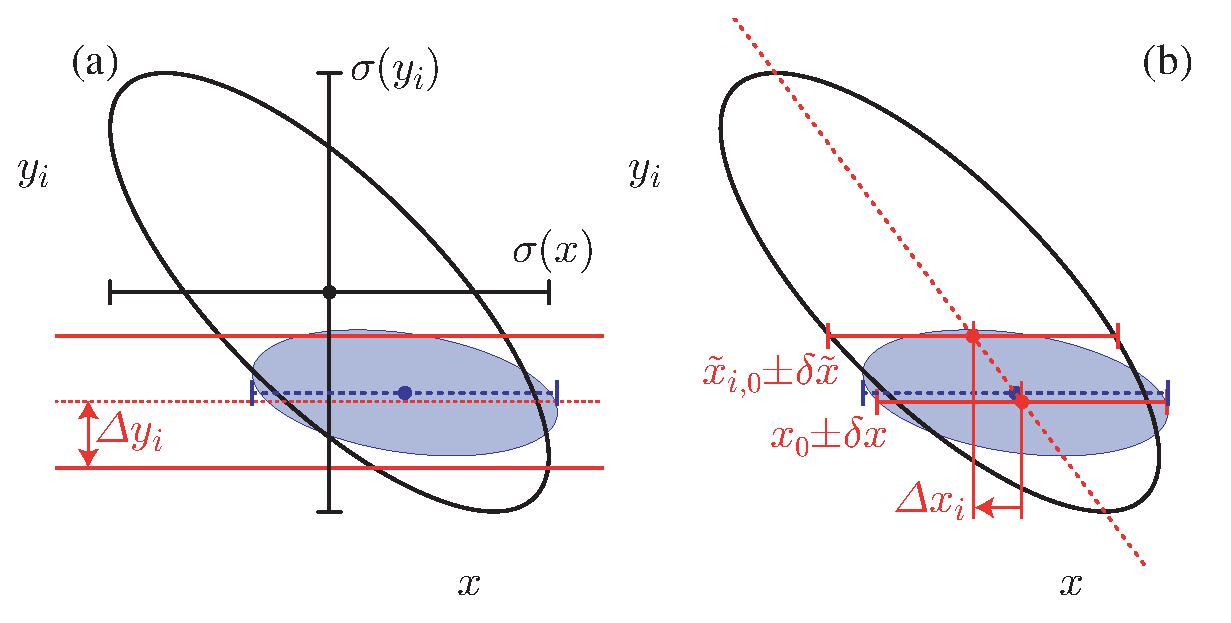
\includegraphics[width=6.0in]{figures/meth/figure1.eps}
\end{center}
\caption{The left-hand plot (a) compares the 68\% confidence-level
  contours of a
  hypothetical measurement's unconstrained (large ellipse) and
  constrained (filled ellipse) likelihoods, using the Gaussian
  constraint on $y_i$ represented by the horizontal band. The solid
  error bars represent the statistical uncertainties $\sigma(x)$ and
  $\sigma(y_i)$ of the unconstrained likelihood. The dashed
  error bar shows the statistical error on $x$ from a
  constrained simultaneous fit to $x$ and $y_i$. The right-hand plot
  (b) illustrates the method described in the text of performing fits
  to $x$ with $y_i$ fixed at different values. The dashed
  diagonal line between these fit results has the slope
  $\rho(x,y_i)\sigma(y_i)/\sigma(x)$ in the limit of a parabolic
  unconstrained likelihood. The result of the constrained simultaneous
  fit from (a) is shown as a dashed error bar on $x$.}
\label{fig:singlefit}
\end{figure}

In practice, the added technical complexity of a constrained fit with
extra free parameters is not justified by the small increase in
sensitivity, as long as the external constraints $\Delta y_i$ are
sufficiently precise when compared with the sensitivities $\sigma(y_i)$
to each $y_i$ of the data alone. Instead, the usual procedure adopted
by the experiments is to perform a baseline fit with all $y_i$ fixed
to nominal values $y_{i,0}$, obtaining $x = x_0 \pm \delta
x$. This baseline fit neglects the uncertainty due to $\Delta y_i$, but
this error can be mostly recovered by repeating the fit separately for
each external parameter $y_i$ with its value fixed at $y_i = y_{i,0} +
\Delta y_i$ to obtain $x = \tilde{x}_{i,0} \pm \delta\tilde{x}$, as
illustrated in Fig.~\ref{fig:singlefit}(b). The absolute shift,
$|\tilde{x}_{i,0} - x_0|$, in the central value of $x$ is what the
experiments usually quote as their systematic uncertainty $\Delta x_i$
on $x$ due to the unknown value of $y_i$. Our procedure requires that
we know not only the magnitude of this shift but also its sign. In the
limit that the unconstrained data is represented by a parabolic
likelihood, the signed shift is given by
\begin{equation}
\Delta x_i = \rho(x,y_i)\frac{\sigma(x)}{\sigma(y_i)}\,\Delta y_i \;,
\end{equation}
where $\sigma(x)$ and $\rho(x,y_i)$ are the statistical uncertainty on
$x$ and the correlation between $x$ and
$y_i$ in the unconstrained data.
While our procedure is not
equivalent to the constrained fit with extra parameters, it yields (in
the limit of a parabolic unconstrained likelihood) a central value
$x_0$ that agrees 
to ${\cal O}(\Delta y_i/\sigma(y_i))^2$ and an uncertainty $\delta x
\oplus \Delta x_i$ that agrees to ${\cal O}(\Delta y_i/\sigma(y_i))^4$.

In order to combine two or more measurements that share systematics
due to the same external parameters $y_i$, we would ideally perform a
constrained simultaneous fit of all data samples to obtain values of
$x$ and each $y_i$, being careful to only apply the constraint on each
$y_i$ once. This is not practical since we generally do not have
sufficient information to reconstruct the unconstrained likelihoods
corresponding to each measurement. Instead, we perform the two-step
approximate procedure described below.

Figs.~\ref{fig:multifit}(a,b) illustrate two
statistically-independent measurements, $x_1 \pm (\delta x_1 \oplus
\Delta x_{i,1})$ and $x_2\pm(\delta x_i\oplus \Delta x_{i,2})$, of the same
hypothetical quantity $x$ (for simplicity, we only show the
contribution of a single correlated systematic due to an external
parameter $y_i$). As our knowledge of the external parameters $y_i$
evolves, it is natural that the different measurements of $x$ will
assume different nominal values and ranges for each $y_i$. The first
step of our procedure is to adjust the values of each measurement to
reflect the current best knowledge of the values $y_i'$ and ranges
$\Delta y_i'$ of the external parameters $y_i$, as illustrated in
Figs.~\ref{fig:multifit}(c,b). We adjust the
central values $x_k$ and correlated systematic uncertainties $\Delta
x_{i,k}$ linearly for each measurement (indexed by $k$) and each
external parameter (indexed by $i$):
\begin{align}
x_k' &= x_k + \sum_i\,\frac{\Delta x_{i,k}}{\Delta y_{i,k}}
\left(y_i'-y_{i,k}\right)\\
\Delta x_{i,k}'&= \Delta x_{i,k}\cdot \frac{\Delta y_i'}{\Delta
  y_{i,k}} \; .
\end{align}
This procedure is exact in the limit that the unconstrained
likelihoods of each measurement is parabolic.

\begin{figure}
\begin{center}
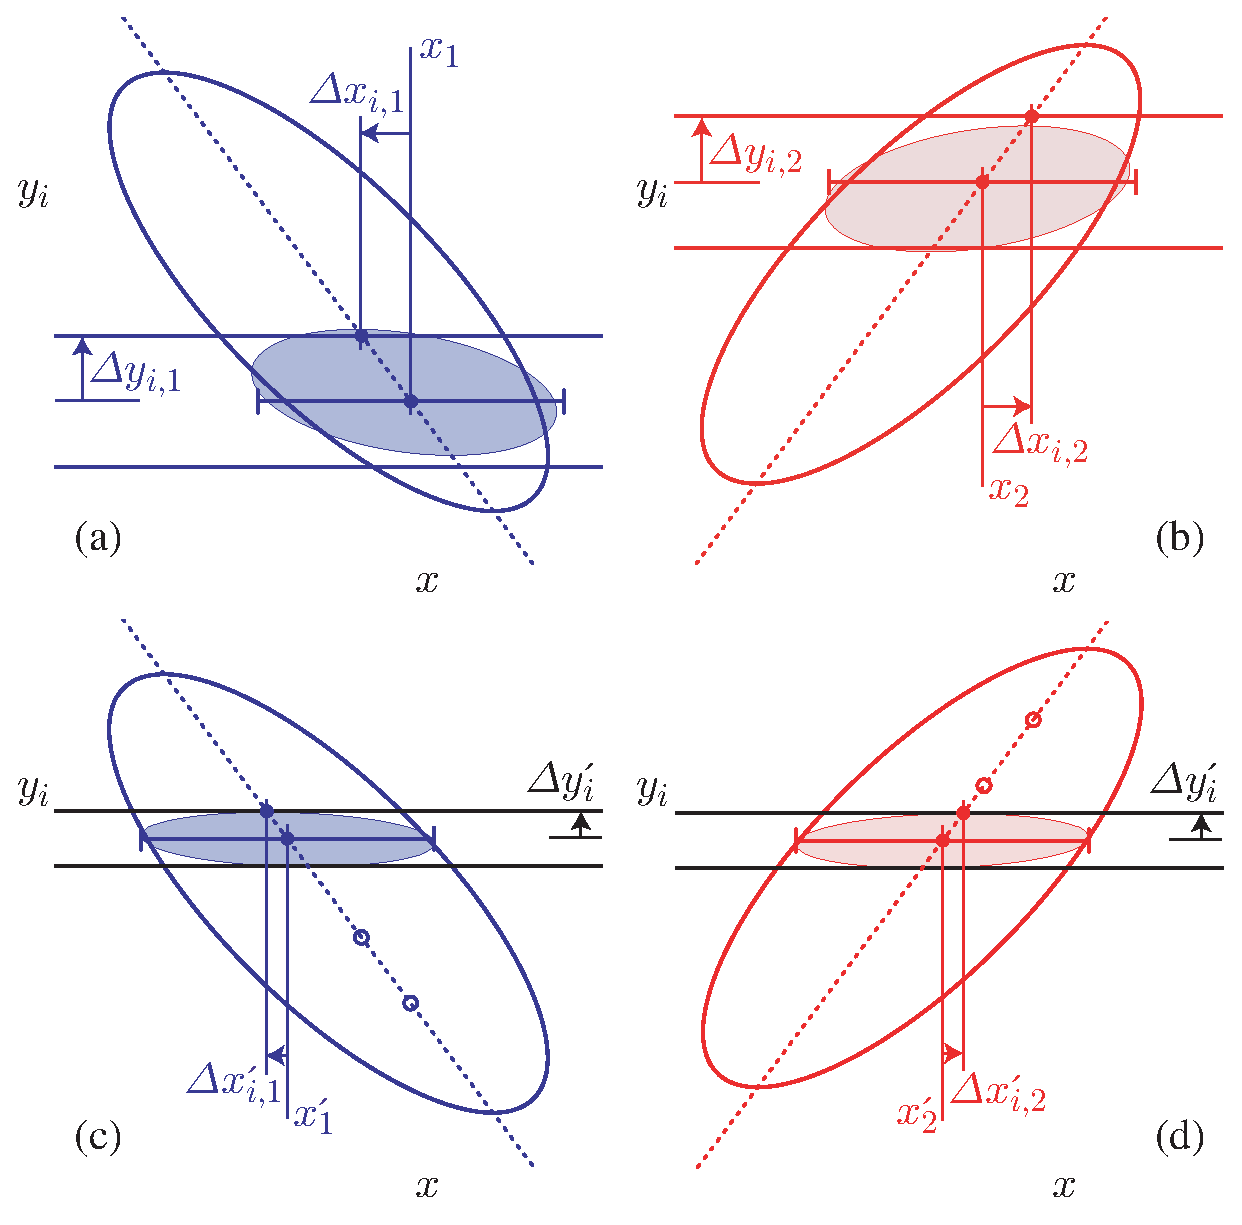
\includegraphics[width=6.0in]{figures/meth/figure2.eps}
\end{center}
\caption{The upper plots (a) and (b) show examples of two individual
  measurements to be combined. The large ellipses represent their
  unconstrained likelihoods, and the filled ellipses represent their
  constrained likelihoods. Horizontal bands indicate the different
  assumptions about the value and uncertainty of $y_i$ used by each
  measurement. The error bars show the results of the approximate
  method described in the text for obtaining $x$ by performing fits
  with $y_i$ fixed to different values. The lower plots (c) and (d)
  illustrate the adjustments to accommodate updated and consistent
  knowledge of $y_i$ as described in the text. Open circles mark the
  central values of the unadjusted fits to $x$ with $y$ fixed; these
  determine the dashed line used to obtain the adjusted values. }
\label{fig:multifit}
\end{figure}

The second step of our procedure is to combine the adjusted
measurements, $x_k'\pm (\delta x_k\oplus \Delta x_{k,1}'\oplus \Delta
x_{k,2}'\oplus\ldots)$ using the chi-square 
\begin{equation}
\chi^2_{\text{comb}}(x,y_1,y_2,\ldots) \equiv \sum_k\,
\frac{1}{\delta x_k^2}\left[
x_k' - \left(x + \sum_i\,(y_i-y_i')\frac{\Delta x_{i,k}'}{\Delta y_i'}\right)
\right]^2 + \sum_i\,
\left(\frac{y_i - y_i'}{\Delta y_i'}\right)^2 \; ,
\end{equation}
and then minimize this $\chi^2$ to obtain the best values of $x$ and
$y_i$ and their uncertainties, as illustrated in
Fig.~\ref{fig:fit12}. Although this method determines new values for
the $y_i$, we do not report them since the $\Delta x_{i,k}$ reported
by each experiment are generally not intended for this purpose (for
example, they may represent a conservative upper limit rather than a
true reflection of a 68\% confidence level).

\begin{figure}
\begin{center}
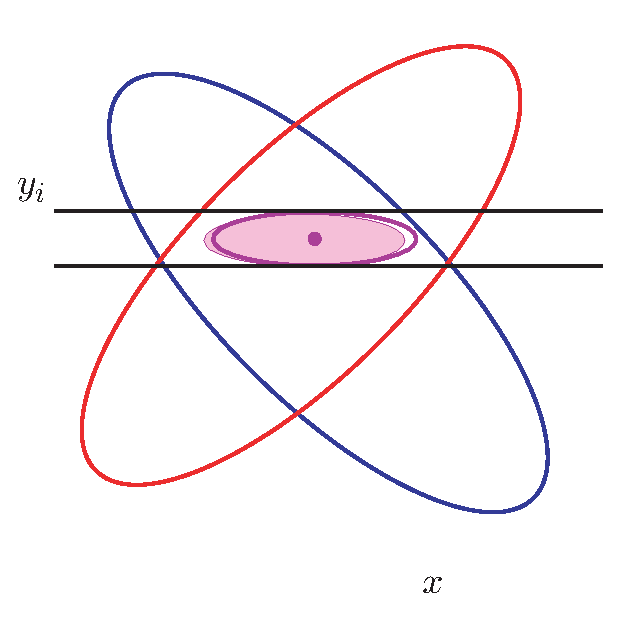
\includegraphics[width=3.5in]{figures/meth/figure3.eps}
\end{center}
\caption{An illustration of the combination of two hypothetical
  measurements of $x$ using the method described in the text. The
  ellipses represent the unconstrained likelihoods of each measurement,
  and the horizontal band represents the latest knowledge about $y_i$ 
  that is used to adjust the individual measurements. The filled small
  ellipse shows the result of the exact method using 
  ${\cal L}_{\text{comb}}$, and the hollow small ellipse and dot show 
  the result of the approximate method using $\chi^2_{\text{comb}}$.}
\label{fig:fit12}
\end{figure}

For comparison, the exact method we would
perform if we had the unconstrained likelihoods ${\cal L}_k(x,y_1,y_2,\ldots)$
available for each
measurement is to minimize the simultaneous constrained likelihood
\begin{equation}
{\cal L}_{\text{comb}}(x,y_1,y_2,\ldots) \equiv \prod_k\,{\cal
  L}_k(x,y_1,y_2,\ldots)\,\prod_{i}\,{\cal 
  L}_i(y_i) \; ,
\end{equation}
with an independent Gaussian external constraint on each $y_i$
\begin{equation}
{\cal L}_i(y_i) \equiv \exp\left[-\frac{1}{2}\,\left(\frac{y_i-y_i'}{\Delta
 y_i'}\right)^2\right] \; .
\end{equation}
The results of this exact method are illustrated by the filled ellipses
in Figs.~\ref{fig:fit12}(a,b) and agree with our method in the limit that
each ${\cal L}_k$ is parabolic and that each $\Delta
y_i' \ll \sigma(y_i)$. In the case of a non-parabolic unconstrained
likelihood, experiments would have to provide a description of ${\cal
  L}_k$ itself to allow an improved combination. In the case of
$\sigma(y_i)\simeq \Delta y_i'$, experiments are advised to perform a
simultaneous measurement of both $x$ and $y$ so that their data will
improve the world knowledge about $y$. 

 The algorithm described above is used as a default in the averages
reported in the following sections.  For some cases, somewhat simplified
or more complex algorithms are used and noted in the corresponding 
sections. Some examples for extensions of the standard method for extracting
averages are given here. These include the case where measurement errors
depend on the measured value, i.e. are relative errors, unknown
correlation coefficients and the breakdown of error sources.

For measurements with Gaussian errors, the usual estimator for the
average of a set of measurements is obtained by minimizing the following
$\chi^2$:
\begin{equation}
\chi^2(t) = \sum_i^N \frac{\left(y_i-t\right)^2}{\sigma^2_i} ,
\label{eq:chi2t}
\end{equation}
where $y_i$ is the measured value for input $i$ and $\sigma_i^2$ is the
variance of the distribution from which $y_i$ was drawn.  The value $\hat{t}$
of $t$ at minimum $\chi^2$ is our estimator for the average.  (This
discussion is given for independent measurements for the sake of
simplicity; the generalization to correlated measurements is
straightforward, and has been used when averaging results.) 
The true $\sigma_i$ are unknown but typically the error as assigned by the
experiment $\sigma_i^{\mathrm{raw}}$ is used as an estimator for it.
Caution is advised,
however, in the case where $\sigma_i^{\mathrm{raw}}$
depends on the value measured for $y_i$. Examples of this include
an uncertainty in any multiplicative factor (like
an acceptance) that enters the determination of $y_i$, i.e. the $\sqrt{N}$
dependence of Poisson statistics, where $y_i \propto N$
and $\sigma_i \propto \sqrt{N}$.
Failing to account for this type of
dependence when averaging leads to a biased average.
Biases in the average can be avoided (or at least reduced)
by minimizing the following
$\chi^2$:
\begin{equation}
\chi^2(t) = \sum_i^N \frac{\left(y_i-t\right)^2}{\sigma^2_i(\hat{t})} .
\label{eq:chi2that}
\end{equation}
In the above $\sigma_i(\hat{t})$ is the uncertainty
assigned to input $i$ that includes the assumed dependence of the
stated error on the value measured.  As an example, consider 
a pure acceptance error, for which
$\sigma_i(\hat{t}) = (\hat{t} / y_i)\times\sigma_i^{\mathrm{raw}}$ .
It is easily verified that solving Eq.~\ref{eq:chi2that} 
leads to the correct behavior, namely
$$ 
\hat{t} = \frac{\sum_i^N y_i^3/(\sigma_i^{\mathrm{raw}})^2}{\sum_i^N y_i^2/(\sigma_i^{\mathrm{raw}})^2},
$$
i.e. weighting by the inverse square of the 
fractional uncertainty, $\sigma_i^{\mathrm{raw}}/y_i$.
It is sometimes difficult to assess the dependence of $\sigma_i^{\mathrm{raw}}$ on
$\hat{t}$ from the errors quoted by experiments.  

%An example is the
%uncertainty on a branching fraction, $\mathcal{B}=(N-B)/\eff$, due to
%a change in the background modeling.   
%As a result, the sensitivity
%to different assumptions on these dependences has been
%studied for the averages given in this section.

Another issue that needs careful treatment is the question of correlation
among different measurements, e.g. due to using the same theory for
calculating acceptances.  A common practice is to set the correlation
coefficient to unity to indicate full correlation.  However, this is
not a ``conservative'' thing to do, and can in fact lead to a significantly
underestimated uncertainty on the average.  In the absence of
better information, the most conservative choice of correlation coefficient
between two measurements $i$ and $j$
is the one that maximizes the uncertainty on $\hat{t}$
due to that pair of measurements:
\begin{equation}
\sigma_{\hat{t}(i,j)}^2 = \frac{\sigma_i^2\,\sigma_j^2\,(1-\rho_{ij}^2)}
   {\sigma_i^2 + \sigma_j^2 - 2\,\rho_{ij}\,\sigma_i\,\sigma_j} ,
\label{eq:correlij}
\end{equation}
namely
\begin{equation}
\rho_{ij} = \mathrm{min}\left(\frac{\sigma_i}{\sigma_j},\frac{\sigma_j}{\sigma_i}\right) ,
\label{eq:correlrho}
\end{equation}
which corresponds to setting $\sigma_{\hat{t}(i,j)}^2=\mathrm{min}(\sigma_i^2,\sigma_j^2)$.
Setting $\rho_{ij}=1$ when $\sigma_i\ne\sigma_j$ can lead to a significant
underestimate of the uncertainty on $\hat{t}$, as can be seen
from Eq.~\ref{eq:correlij}.

Finally, we carefully consider the various sources of error
contributing to the overall uncertainty of an average.
The overall covariance matrix is constructed from a number of
individual sources, e.g.
$\mathbf{V} = \mathbf{V_{stat}+V_{sys}+V_{th}}$.
The variance on the average $\hat{t}$ can be written
\begin{eqnarray}
\sigma^2_{\hat{t}} 
 &=& 
\frac{ \sum_{i,j}\left(\mathbf{V^{-1}}\, 
\mathbf{[V_{stat}+V_{sys}+V_{th}]}\, \mathbf{V^{-1}}\right)_{ij}}
{\left(\sum_{i,j} V^{-1}_{ij}\right)^2}
= \sigma^2_{stat} + \sigma^2_{sys} + \sigma^2_{th} .
\end{eqnarray}
Written in this form, one can readily determine the 
contribution of each source of uncertainty to the overall uncertainty
on the average.  This breakdown of the uncertainties is used 
%below.
in the following sections.

Following the prescription described above, the central values and
errors are rescaled to a common set of input parameters in the averaging
procedures according to the dependency on any of these input parameters.
We try to use the most up-to-date values for these common inputs and 
the same values among the HFAG subgroups. For the parameters whose
averages are produced by HFAG, we use the values in the current 
update cycle.  For other external parameters, we use the most
recent PDG values available (usually Ref.~\cite{PDG_2010}). 
The parameters and values used are listed in each subgroup section.
